\chapter{Introduction}
\label{chap:introduction}

{ \Large \leftwatermark{
\put(-76.5,-75){
\includegraphics[scale=0.8]{img/thumbindex.eps}}  \put(-67,-66.5){ {\color{white} 1 }}
\put(-67,-91.5){ 2 }
\put(-67,-116.5){ 3 }
\put(-67,-141.5){ 4 }
\put(-67,-166.5){ 5 }
\put(-67,-191.5){ 6 }
\put(-67,-216.5){ 7 }
\put(-67,-241.5){ 8 }
} \rightwatermark{
\put(346.5,-75){
\includegraphics[scale=0.8]{img/thumbindex.eps}}  \put(350.5,-66.5){ {\color{white} 1 }}
\put(350.5,-91.5){ 2 }
\put(350.5,-116.5){ 3 }
\put(350.5,-141.5){ 4 }
\put(350.5,-166.5){ 5 }
\put(350.5,-191.5){ 6 }
\put(350.5,-216.5){ 7 }
\put(350.5,-241.5){ 8 }
}}

\newpage

\noindent
Translational medical genetics is a cross-disciplinary field of research that strives to advance genomic medicine using state-of-the-art findings from life sciences.
In this thesis, I contribute bioinformatic models, methods and systems to improve the rate and precision of patient diagnoses by harnessing untapped molecular information.

I start this introduction by discussing the origins of the field of genetics and how it evolved to its current state (\ref{intro_origin}).
I then zoom in on medical genetics and explain how our growing understanding of genetic disorders benefits patients (\ref{intro_clingen}).
Recent revolutions in DNA sequencing now allow us to complement genetics with genomics, which is the physical characterization of the genome itself.
I explain how this shift presents medical practice with many exciting opportunities but also with equally big challenges (\ref{intro_bioinfchall}) for successful implementation.
These challenges that feed into the research questions addressed in this thesis (\ref{intro_bioinfopp}).
The introduction ends with an overview of the chapters of this thesis (\ref{intro_outline}).
Each chapter presents research that aims to translate these opportunities into better understanding, diagnosis, and ultimately treatment of genetic disorders.

\section[The origin of genetics]{The origin of genetics: solving the genetic riddle piece by “peas”} \label{intro_origin}

Just over 150 years ago, Gregor Mendel was the first to describe the basic rules of genetic inheritance\cite{Mendel_1866}.
He discovered striking patterns in how the traits of pea plants such as color and shape were transmitted from one generation to the next.
His work established genetics as a science, even though he could not know the molecular basis of his observations.

It was only decades later that Mendel’s theories were finally recognized, and the term \textsl{gene} was coined\cite{Johannsen_1909} as an innate unit of inheritance.
Genes were defined as the effect observed on the traits (i.e. \textsl{phenotype}, these and other terms are clarified in Tables \ref{table:introduction_glossary_1} and \ref{table:introduction_glossary_2}), and were not yet measured on a molecular level.

Traits may be passed on to the next generation independently from each other, but some traits seemed to be passed on together with a certain frequency.
The relative distance of the underlying genes could be estimated by analyzing this effect, called \textsl{linkage}\cite{Morgan_1915}, although it was only realized much later that this is related to physical distance on a DNA molecule.
Further studies showed that genes seemed to direct en\-zyme syn\-the\-sis\cite{Beadle_1941} and that nucleic acid was the carrier of genetic material\cite{Avery_1944,Hershey_1952}, not proteins, as was the popular belief\footnote{Nevertheless, there are known mechanisms for protein-based inheritance\cite{Prusiner_1998,Chakrabortee_2016} and cell memory\cite{Caudron_2013}.}.

How the information of genes was stored in nucleic acid was unclear until the physical structure of DNA was elucidated\cite{Watson_1953}.
This was followed by the cracking of the genetic code\cite{Leder_1964}, specifically how DNA codon triplets are translated via temporary RNA-based copies into amino acid sequences that fold into functional proteins.
These proteins are the workhorses of the cell. They communicate with other cells (e.g. via excretions and receptors), process metabolic substrates (e.g. via glycolysis) and regulate cell homeostasis (e.g. via signal transduction).

The first completely sequenced genome was that of a virus, Bacteriophage MS2, which has just 3,569 DNA bases\cite{Fiers_1976}.
When the human genome sequence was completed in the year 2000\cite{Lander_2001}, it turned out to have over 3,000,000,000 base pairs\footnote{The largest reliably measured genome currently known belongs to the Japanese Canopy plant \textsl{P. japonica}, which has ~150,000,000,000 base pairs\cite{Pellicer_2010}.}.
With this milestone, the field of human molecular genetics gained huge momentum.
Now, traits and diseases could be associated to the actual sequence of DNA instead of an abstract linkage map or approximate cytogenetic location (observable chromosomal aberrations leading to a disease phenotype).

\begin{table}
\begin{tabulary}{\linewidth}{LL}
  \mbox{Term~~~~~~~~~~~~~~~~~~~~~~~~~~~~~~~~~~~~} & Definition \\
  \hline
  \rule{0pt}{2.5ex}Allele & A variant form of a gene or genetic locus \\
  \rule{0pt}{2.5ex}Amino acid & Small organic building block of proteins \\
  \rule{0pt}{2.5ex}Base & Building block of nucleic acid \\
  \rule{0pt}{2.5ex}Base pair & Two bases bound by hydrogen in the DNA double helix \\
  \rule{0pt}{2.5ex}Chromosome & Organizational unit of DNA, humans have 22 pairs plus XX or XY \\
  \rule{0pt}{2.5ex}Codon triplet & Sequence of three bases that codes for a specific amino acid \\
  \rule{0pt}{2.5ex}Complex disease & A disease caused by the joined effect of multiple environmental and genetic factors \\
  \rule{0pt}{2.5ex}Conserved loci & Genomic locations that have changed little in evolution \\
  \rule{0pt}{2.5ex}Diagnostic yield & The percentage of solved patient cases \\
  \rule{0pt}{2.5ex}DNA & Deoxyribonucleic acid, encodes the genetic information of an organism \\
  \rule{0pt}{2.5ex}Dominant disease & A disease caused by a single pathogenic allele on one chromosome of a pair \\
  \rule{0pt}{2.5ex}Enzyme synthesis & Production of proteins that act in, or execute chemical reactions \\
  \rule{0pt}{2.5ex}Exon & Short for 'expressed region', coding sections of a DNA sequence \\
  \rule{0pt}{2.5ex}Genetic code & Rules by which nucleic acid is translated into messenger RNA \\
  \rule{0pt}{2.5ex}Genetic inheritance & Transmission of inborn traits from parent to offspring \\
  \rule{0pt}{2.5ex}Genome sequencing & Determining the order of bases in a genome \\
  \hline
\end{tabulary}
\caption[Glossary of key terms, pt. 1/2.]{\label{table:introduction_glossary_1} Glossary of key terms used in this introduction, pt. 1/2.}
\end{table}

\begin{table}
\begin{tabulary}{\linewidth}{LL}
  \mbox{Term~~~~~~~~~~~~~~~~~~~~~~~~~~~~~~~~~~~~~~~~~~~~~~~~~~~~~~~~~~~~} & Definition \\
  \hline
  \rule{0pt}{2.5ex}Homeostasis & Active regulation to maintain a stable equilibrium of variables in an organism \\
  \rule{0pt}{2.5ex}Mendelian inheritance & Set of rules for the basic modes of inheritance for single-gene diseases \\
  \rule{0pt}{2.5ex}Mutation & A change of the nucleotide sequence of the genome \\
  \rule{0pt}{2.5ex}Non-Mendelian inheritance & More complex inheritance patterns such as additive, co-dominance, polygenic, imprinting or heterosis \\
  \rule{0pt}{2.5ex}Nucleic acid & Biopolymer consisting of sugars, phosphates and nitrogenous bases \\
  \rule{0pt}{2.5ex}Oligogenic & A few genes controlling a trait \\
  \rule{0pt}{2.5ex}Penetrance & The proportion of individuals adversely affected by a pathogenic mutation \\
  \rule{0pt}{2.5ex}Phenotype & Collection of observable characteristics of an organism resulting from the interaction of its genotype with the environment \\
  \rule{0pt}{2.5ex}Polymorphism & A neutral and commonly present mutation \\
  \rule{0pt}{2.5ex}Proteins & Large biomolecules with a variety of functions \\
  \rule{0pt}{2.5ex}Recessive disease & A disease caused by pathogenic alleles on both chromosomes of a pair \\
  \rule{0pt}{2.5ex}RNA & Ribonucleic acid, predominantly acts as a messenger carrying instructions from DNA for controlling protein synthesis \\
  \rule{0pt}{2.5ex}Splicing & The process by which exons are joined to form messenger RNA \\
  \rule{0pt}{2.5ex}Variant & General term for all mutations and polymorphisms \\
  \hline
\end{tabulary}
\caption[Glossary of key terms, pt. 2/2.]{\label{table:introduction_glossary_2} Glossary of key terms used in this introduction, pt. 2/2.}
\end{table}


\section{The genome in the clinic} \label{intro_clingen}
Inheritance patterns of inborn disorders in humans have been studied since the rediscovery of Mendel's work, with study focusing mainly on genes.
The first inborn disorder to be described was al\-kap\-to\-nu\-ria\cite{Garrod_1902}, a recessive disease with a pre\-va\-len\-ce of 1:100,\-000 to 1:250,\-000\cite{Zatkova_2011} caused by mutations (i.e. \textsl{variants}, small genetic differences) in the \textsl{HGD} gene on chromosome 3.
There are now around 8,000 such gene-related disorders catalogued in the OMIM\cite{Hamosh_2000}, Orphanet\cite{Orphanet} and DECIPHER\cite{Firth_2009} databases.
For about 4,300 of these disorders an associated gene has been discovered, of which 3,300 are characterized as clinically actionable to some degree\cite{Solomon_2013}.

The majority of clinical genes currently known usually follow a Men\-de\-li\-an inheritance pattern, because those are more straightforward to discover and characterize.
These Mendelian disease genes are traditionally discovered by investigating the transmission pattern of specific mutations through a family pedigree.
The top candidates for these confirmation studies are usually rare mutations at conserved genomic loci that strongly coincide with being affected by the disease.
After more independent families or patients have been found with the same symptoms and the same mutation or affected gene\cite{Sobreira_2015}, a causal relation is established\cite{Cnossen_2014}.

Finding causal genes is not a trivial effort and additional difficulty may be introduced by oligogenic inheritance\cite{Gazzo_2015}, incomplete pe\-ne\-tran\-ce\cite{Shawky_2014,Natarajan_2016}, or variants that have an unexpected effect\cite{Eriksson_2003}.
Causal mutations and genes are catalogued in databases such as Clinical Genomics Database\cite{Solomon_2013} and ClinVar\cite{Landrum_2013}.

Knowing which genes are responsible for disorders provides many opportunities to improve patient care through applications such as improved disease diagnosis, carrier screening, personalized medicine and life course advice.

Firstly, we can use genomic knowledge for more accurate \textbf{disease diagnosis}.
For example, there are five subtypes of cardiomyopathies, with over 60 genes involved\cite{Jongbloed_2010}. Gene sets specific for a given disease type are called \textsl{panels}.
Gene screening panels have been created for conditions including dystonia, dermatology, autoinflammatory diseases, epilepsy, familial cancer, intellectual disability and metabolic disorders.
Finding a pathogenic mutation in one of these genes may lead to a diagnosis on the molecular level, which is more precise than a diagnosis based only on symptoms.

The second opportunity to improve healthcare is through \textbf{carrier screening}, which assesses whether a person is carrying a specific patho\-gen\-ic mutation present in their family.
A special case of carrier screening is preconception screening where it is determined whether both parents carry alleles in the same gene known to cause severe recessive disease.
In this case the parents are not at risk, but a potential child has - following Mendelian laws - a 25\% chance of inheriting both alleles, and thus being affected.

Lastly, \textbf{personalized medicine} refers to better tailoring of medication and treatment based on the genotype of the patient.
A well-known example is the adjustment of the starting dose of warfarin depending the patient's \textsl{CYP2C9} and \textsl{VKORC1} genes\cite{Limdi_2008,Ventola_2011}, which affect their ability to metabolize this drug.

While DNA analysis was very costly until recently, which limited analysis to one or a few genes, clinical geneticists can now perform DNA-sequencing on their patient using a panel of many genes, or choose to look at all 26,000 genes at once using whole-exome sequencing (WES), or even consider whole-genome sequencing (WGS), thanks to \textsl{next-generation DNA-sequencing} techniques (NGS), which has largely replaced more traditional techniques such as Sanger sequencing\cite{Sanger_1977}.
The cost of sequencing a genome with NGS has dropped dramatically, from \$10 million in 2007 to only \$1,000 in 2015\footnote{\url{https://www.genome.gov/sequencingcostsdata/}}, paving the way for a genomic revolution.

WES allows us to investigate thousands of genes at once in research or diagnostics\cite{Yang_2013}.
This technique is useful for making a genome-driven diagnosis when symptoms are hard to assess, for example in newborns\cite{van_Diemen_2017} and other isolated cases\cite{Wilfert_2016}.
WES allows analysis of exons and corresponding splice-site regions.

Using WGS we can look at 'non-coding' DNA, which is not transcribed to protein but is still involved in the regulation of genes.
From application of WGS we now know that non-coding variants are also implicated in disease\cite{Javierre_2016} and that the genome is organized in topological domains\cite{Dixon_2012}, structural changes in which are linked to pathogenic effects\cite{Franke_2016}.
This relatively new area of genomic research is already becoming of diagnostic relevance\cite{Smedley_2016}.

Regardless which technique is used, a molecular diagnosis provides an unprecedented ability to help patients.
Most notably, a diagnosis can be established long before symptoms have developed, allowing recognition and sometimes intervention that may prevent permanent damage\cite{Saunders_2012}.
In all cases, a more informed diagnosis will lead to a clearer prognosis and more appropriate treatment plan based on the molecular etiology of the disease.
However, when using genome-wide screening approaches, incidental findings have to be dealt with\cite{Green_2013b}, as they can cause serious issues including a high patient opt-out rate\cite{Harris_2016}.

\section{Data interpretation challenges} \label{intro_bioinfchall}

Although genetic screening is successfully employed in many clinics around the world, we now effectively use only a minute amount of the genetic knowledge contained within the data generated.
For most of the genes, and for almost all of the non-coding genome, we do not know the clinical relevance.
A genetic cause has been established for only about half of the known Mendelian disorders, and we are only just starting to understand complex diseases\cite{McCarthy_2008}.
Even within the known genes, it is not always clear if a mutation is harmful\cite{Cooper_2015,Chen_2016}.
As a result, the interpretation and subsequent classification of DNA variants is a major challenge.

The difficulty of this challenge is shown by the diagnostic yields currently achieved, which vary from 15 to 80\%\cite{Wang_2014, Mart_nez_2016, Daoud_2016, Yubero_2016} depending on factors such as disease type, patient inclusion criteria and sequencing technique used.
This challenge is further shown by the discordant results given by direct-to-consumer genomic analysis companies\cite{Corpas_2015} and by the re-classification of pathogenic variants as harmless when more data becomes available\cite{Cassa_2013}.

Furthermore, the production of genomic data is far outpacing the rate at which geneticists can interpret it, a circumstance referred to as the 'NGS data deluge'\cite{Schrijver_2012}.
Big data analytics is thus a major challenge in healthcare\cite{Raghupathi_2014,Belle_2015}, as are related efforts to translate research data and research findings into healthcare improvements\cite{Alyass_2015,Auffray_2016}.
This is especially true for the area of medical genetics\cite{Ginsburg_2014,Wang_2014b,Bowdin_2014}.
Adding more layers of molecular information, such as transcriptomics or epigenetics, only makes sense when combined with infrastructure and analysis methods that use these data to make clinical decisions easier instead of more complicated.

Computers can help us integrate and analyze large and complex data, provided appropriate software is available to do so.
The field of bioinformatics develops these tools, but it takes more than a few lines of code to improve patient care.
This barriers for setting up infrastructure can be broken down into effective data integration, method development and implementation into practice.
In this thesis we identify and address the following challenges:

\begin{enumerate}
  \item We need data \textbf{models} to integrate life science data for genetic disease research. By systematically integrating and visualizing large a\-mounts of data sets, we allow researchers to discover new disease genes. These genes can then be tested in patients, leading to higher diagnostic yield.
  \item We need computational \textbf{methods} to translate research findings to medical genetics. Many research findings are of potential benefit to patient care, but they require tailoring, calibration and validation into a clinical genomics context before they can be used. Using more advanced analysis methods will result in more accurate and efficient characterization of patient mutations.
  \item We need software \textbf{systems} to implement methods into medical genetics practice. These systems are needed to test, validate and utilize new methods and must be flexible enough to allow quick adoption of future developments, including new methods and data modalities.
\end{enumerate}

\section{Bioinformatic opportunities} \label{intro_bioinfopp}

Empowering clinical geneticists with the tremendous amount and variety of new life science data is the huge challenge that forms the objective of this thesis. 
Basic science in biology and genetics includes studies on model organisms, human populations, creation of computational algorithms and the molecular characterization of cells and tissues, and all these types of research present possibilities to improve patient diagnoses.
At the same time, medical practice offers invaluable insights about disease etiology, patient cases, and data gathered in a clinical setting that can be used to develop and validate new methods for medical application.
All these new data offer major opportunities for finding, understanding and treating human disease.
Figure \ref{fig:introduction_overview} illustrates the efforts and collaborations in the translational research needed to realize this potential.
In the paragraphs below and more detailed sections devoted to them that follow, we introduce the key research topics that are the focus of this thesis:

\begin{figure}
\centering
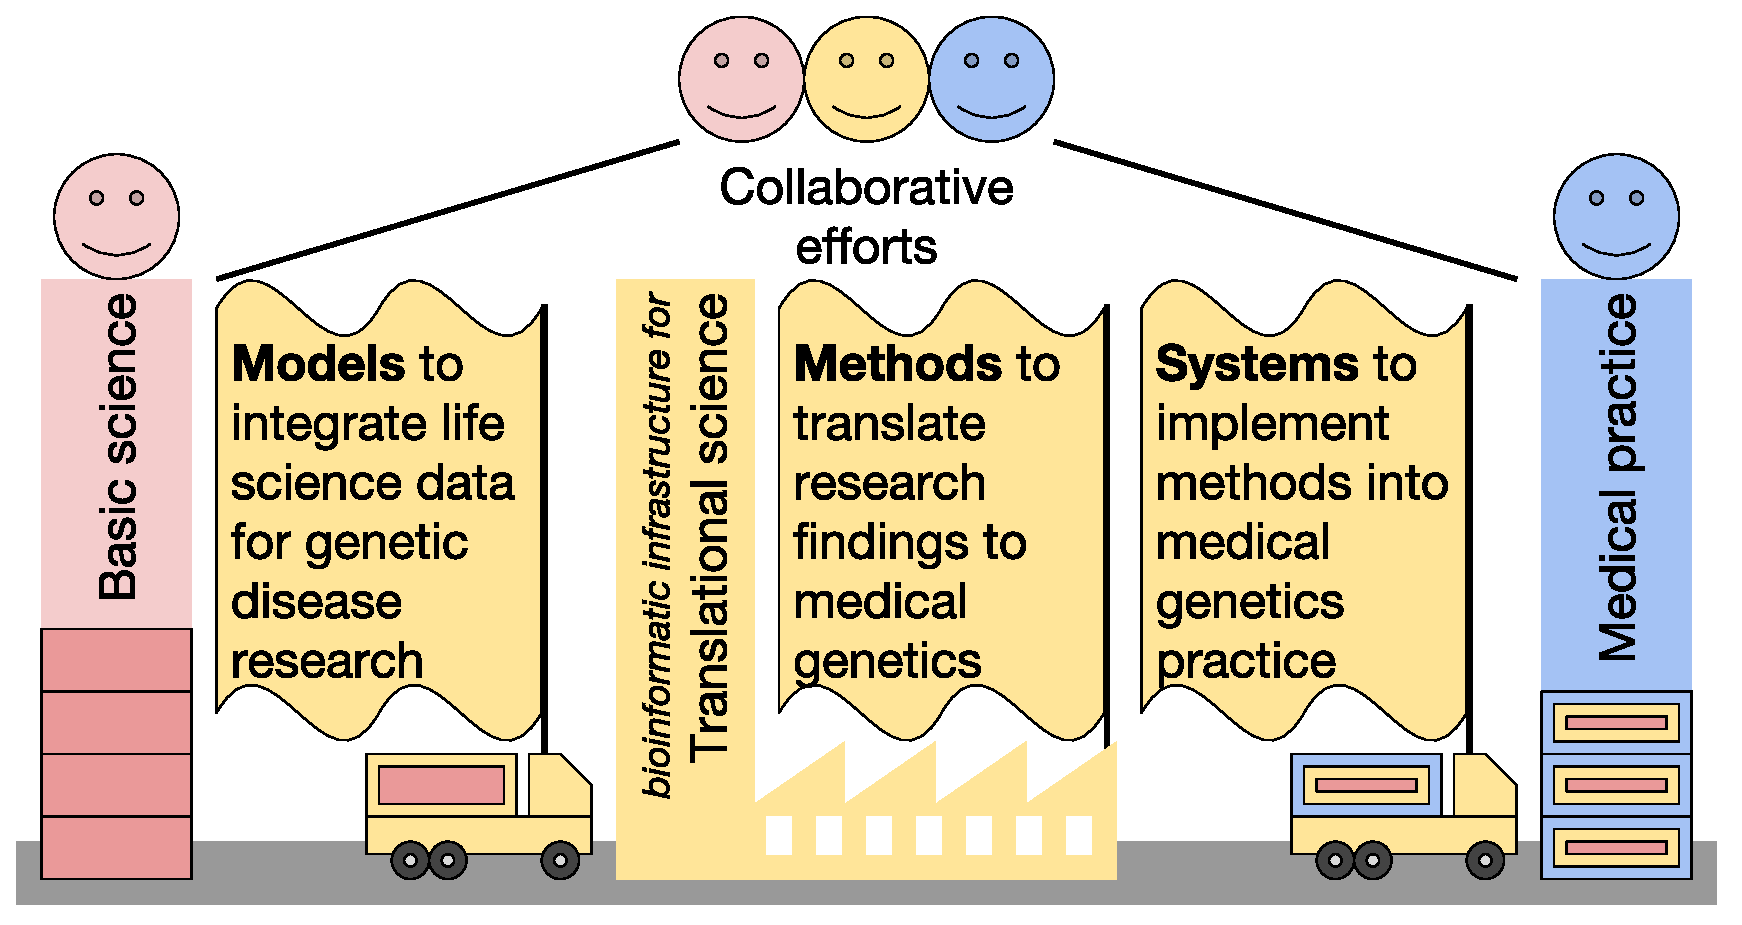
\includegraphics[width=1.0\linewidth]{img/introduction_overview}
\caption[Translational science overview]{Overview of bioinformatic infrastructure for translational science. Fundamental knowledge originates in basic research (red). Translational research (yellow) bridges the gap between basic research and medical practice (blue) by collaborative efforts from all parties involved.}
\label{fig:introduction_overview}
\end{figure}

Reference genomes - Population studies can tell us what to expect in the average individual.
Through phenotypic and molecular characterization of large groups of healthy individuals, we can establish a reference population.
Strong deviation from this reference may point towards causal mechanisms of molecular disease for more severe disorders that are highly damaging or otherwise debilitating at a younger age.

Association studies - Patient studies can tell us how disorders originate.
While studying small numbers of individuals can still uncover new Mendelian disease genes\cite{Witteveen_2016}, larger number of patients are required for statistical association of new disease candidate genes with less obvious effects\cite{Lelieveld_2016}.
By using extremely large sample sizes, we can also detect genetic associations for complex but more common afflictions such as celiac disease or obesity.

Additional molecular data - The genome is the prime information carrier within a living cell, but many more molecular levels stand between the DNA sequence and the eventual expression of a phenotype.
By measuring these different levels we can attempt to reconstruct both the lateral interactions (protein-protein interactions or gene co-expression networks) and perpendicular interactions (protein binding to the genome to silence expression or metabolite accumulation causing neurodegeneration), which can help to understand the workings of disease in detail.

Computational and 'big data' approaches - The rich collection of current life science data provides great opportunities for the development of smart software programs, computational algorithms and statistical tools that can extract knowledge from these growing data resources.
These must perform a multitude of roles and functions, including cleaning and quality control of raw data, imputing missing data points, finding statistical associations, modeling and running predictors, or constructing and pruning networks of detected relations.
In the following paragraphs I will explore these opportunities in detail.

\subsection{Population reference genomes}
Genomes are relatively similar between individuals, therefore, instead of assembling the complete sequence for each person, we only determine points of DNA variation compared to a reference genome.
Subsequently, we can aggregate the results by counting how often each point of variation was observed.
This allows us to store the information of thousands of genomes in files that are still quite computationally manageable and require smaller amounts of data storage capacity.
There are a number of initiatives that have collected the DNA variation of healthy individuals, such as the Thousand Genomes project\cite{McVean_2012} (2,504 genomes), the Genome of the Netherlands\cite{Francioli_2014} (750 genomes), the Exome Aggregation Consortium\cite{Lek_2016} (60,706 exomes), the NHLBI Exome Sequencing Project\cite{EVS} (6,503 exomes) and the upcoming gnomAD from the ExAC authors\cite{Lek_2016} (126,216 exomes and 15,137 genomes).
Here, the term “healthy” refers to individuals who do not suffer from a severe inborn disorder.
They may still develop common late-onset diseases with genetic components such as type 2 diabetes, cardiovascular problems, obesity or common forms of cancer.

These large reference sets find eager uptake in all areas of genetics including research and genome diagnostics.
Variants observed to have a high allele frequency in a population of individuals are called polymorphisms.
Such polymorphisms are very unlikely to directly cause a disease, although they might still act as modifiers (or markers) for disease risk\cite{Donald_2017}.
We may apply a filter based on Minor Allele Frequency (MAF): the alternative allele fraction compared to the most frequent reference allele.
A typical setting may be to exclude any variant from further analysis of a patient's genome when it occurs more than 1\% in the general population.
Depending on the rarity and severity of a disease, we may want to use thresholds as low as 0.01\% (see chapter \ref{chap:gavin}) and as high as 5\%\cite{Strom_2011}.
We can also use the genotype zygocity counts, which is the number of individuals heterozygous or homozygous for an allele.
If only heterozygous genotypes are observed in the general healthy population, we may be dealing with a recessive-acting disease variant, which quickly becomes a candidate for being pathogenic when detected homozygously in a patient.

As other types of population reference data becomes available, e.g. from RNA-sequencing\cite{Deelen_2015}, we have the opportunity to also establish a baseline for healthy individuals for data other than DNA variation.
We can use these references to investigate and manually predict potential pathogenic effects in patients and capture the outcomes.
These results are then used to develop tools to speed up the interpretation of new patient data and initiate a synergistic process leading to exponential tool development.

Furthermore, big population data provide insight into our genomic architecture.
The mention of Mendelian disease genes may give the impression that our genomes are fragile, but there is also evidence that shows they are surprising resilient.
Each healthy human has about 100 Loss of Function (LoF) variants with ~20 genes completely in\-ac\-ti\-va\-ted\cite{MacArthur_2012}.
We now have enough reference data to calculate an accurate LoF rate for every gene\cite{Lek_2016}, and this rate may be compared to a null distribution to determine which genes are LoF-tolerant and which are not. 
Any LoF-intolerant genes found in patients with severe mutations can then be prioritized as potentially disease-causing.
By analyzing the selection pressure on truncating variants we can then characterize genes, and estimate whether one or two dysfunctional alleles are likely to be disease causative\cite{Cassa_2017}.

Lastly, these large reference sets have put things in new perspective.
Some variants that were previously thought to be surely disease-causing were found to have low \textsl{penetrance}, meaning that not every individual with that mutation actually becomes ill\cite{Minikel_2016}.
Other variants once thought to have pathogenic effects have turned out to be far too common with respect to disease prevalence, revealing them as false positives\cite{Walsh_2016}.
Finally, on a more critical note, ethnicity biases in these reference sets may result in misclassifications\cite{Manrai_2016}, indicating a need for more diverse and representative data sets to be used in genome diagnostic interpretation.

\subsection{Genomic association studies}
In Mendelian or \textsl{monogenic} genetic disorders, a single dysfunctional gene can cause severe problems.
There are, however, numerous disease-related phenotypes that are not attributable to just one or a few genes.
Instead, many locations (or \textsl{loci}) on the genome seem to each contribute a small amount to the risk of the disease\cite{McCarthy_2008,Manolio_2009,Boyle_2017}.
Finding these weak associations requires large Genome-Wide Association Studies or \textsl{GWAS} which may include more than 250,000 participants\cite{Wood_2014}.
These large samples sizes can be achieved by genotyping arrays which can cheaply ascertain alleles of a predetermined set of variants.

In human, we have currently discovered about 30,000 trait-genome associations\cite{Welter_2013}.
While these include general traits like word reading ability, alcohol consumption, hair color, height, and freckling, most traits are of medical relevance and include susceptibility to common diseases such as hypertension, arthritis, celiac disease, cancer subtypes, diabetes, cardiovascular disease, ulcerative colitis, obesity, allergies, psoriasis and asthma.

Establishing these associations is important for several reasons.
Most notably, the locations where they are found implicate nearby genes that may be involved, making these genes the best candidates for further study.
However, genes must be carefully considered because the closest gene is often not relevant and statistical approaches have been developed\cite{Zhu_2016} to identify the strongest candidate in the region.

Another application of GWAS associations is modeling of genetic risk scores.
The effect size of the risk-associated alleles that an individual is harboring can be summed to a genetic risk score\cite{Dudbridge_2013}.
This risk, by definition, correlates to either the chance of developing a certain disease or the occurrence of a clinical event\cite{Malik_2014}, but genetic risk scores can also predict the quantitative severity of a clinical phenotype\cite{Belsky_2013}.

Based on a higher risk score, individuals may choose to undergo a specific medical check regularly, or adjust their lifestyles to improve their odds of not developing a certain disease.
Conversely, individuals with strong protective alleles might need fewer periodic examinations than usual, allowing physicians to spend more time on people with a higher risk.

\subsection{Additional molecular data}

Beyond the DNA sequence, much additional molecular data can now be gathered that can be used to identify which DNA variations are relevant for health and disease, and which are not.
Regulation of gene transcription, translation, protein activity and degradation constantly takes place at between different molecular levels.
For instance, the genes on the genome itself can be made harder to transcribe through methylation of the cytosine and adenine nucleotides\cite{Bird_2002}.
In addition, the chromosomal structure of DNA can be decondensated by histone acetylation (transfer of acetyl groups to DNA organizational elements), making it more accessible for transcription\cite{Eberharter_2002}.
The transcriptional expression of genes is further regulated by genetic variants themselves\cite{Albert_2015}.
Finally, proteins form a complex network of interactions\cite{Phizicky_1995} that, in turn, also regulate gene expression\cite{Taniguchi_2012}.

We study the complex patterns of this regulation to understand how genes act in concert, and how a disease phenotype presents in cells, tissues and organisms.
Large initiatives that pursue this goal include studies into expression quantitative trait loci (eQTL)\cite{Westra_2013} and allele-specific expression\cite{Deelen_2015}, characterization of functional genomic elements including methylation and acetylation patterns\cite{Dunham_2012}, comprehensive expression studies across different tissues\cite{Lonsdale_2013} and cell types\cite{Forrest_2014}.

These same kinds of studies can also be performed on model organisms, which can be bred and measured in highly controlled environments for pin-point phenotypic and molecular characterization.
Studies on mice have been an essential tool for biological research for more than a century and continue their important role today\cite{Phifer_Rixey_2015}.
Mice are evolutionarily relatively close to humans, and their size and short generation time allows experiments to be set up and run with large enough numbers for statistical significance.
However, other types of model organisms such as zebrafish\cite{Lieschke_2007} and worm\cite{Kaletta_2006} can offer unique advantages over using rodents.
While these organisms have a larger evolutionary distance to humans, they are cheaper, faster and easier to breed and have transparent bodies that are easy to dissect.
The tiny \textsl{C. elegans} worm has by far the fastest life cycle, simplest anatomy and the unique property of strains that can be frozen and revived.

In addition to transcriptomics and epigenetics, we can also measure the levels of metabolites and proteins present in cells.
These technologies, known as metabolomics and proteomics, can be integrated with genomics data\cite{Grapov_2015} to obtain a more complete understanding of the complex processes in the cell that interplay with all these layers.
Finally, we can also investigate the genomic variation that prevents disease or even increase our health instead of looking for genes that make people ill.
The search for so-called 'protective alleles' is an up and coming area of study that will also result in healthcare advancements\cite{Harper_2015}.

\subsection{Computational and 'big data' approaches}

Measuring and interpreting the large, complex and diverse life-science datasets has driven the development of a plethora of new computational methods and tools to analyze these data.
These include methods to clean and prepare data for analysis, advanced statistical methods, relational databases, web applications, data integration and visualization tools.

A few notable examples include the Variant Quality Score Recalibration (VQSR), a module of the Genome Analysis Toolkit (GATK)\cite{Van_der_Auwera_2013}.
This tool performs comparative machine learning on identified (\textsl{called}) NGS variants versus a reference truth set to find the optimal variables for determining which variants are true positives and which are false.

Variants can also be determined using genotyping platforms, but when multiple platforms are used, data are not comparable.
However, they can be harmonized by inferring missing variants using genotype imputation\cite{Deelen_2014}, which also uses reference knowledge.

After variants are determined, there are many tools that estimate variant pathogenicity to assist genome diagnostics or research into genetic diseases\cite{Eilbeck_2017}.
A powerful method to prioritize variants for further interpretation are CADD scores\cite{Kircher_2014}.
These scores are a measure of evolutionary pressure on genetic variants that builds upon 60+ existing tools and sources.
Variants with a higher score are more likely to be deleterious and are therefore the best candidates in disease research.

Using CADD scores, variants are discovered in genes of which the function is not yet known.
Knowledge net\-works such as Gene\-MA\-NIA\cite{Warde_Farley_2010} may help to infer a putative function by linking unknown genes to genes known from previous studies to show a similar expression pattern.
We can also characterize unknown genes by their evolutionary, loss-of-function and network interaction properties to prioritize candidate variants\cite{Khurana_2013} and even predict disease inheritance mode to a certain degree\cite{Hsu_2016}.

Taking this approach a step further, GeneNetwork\cite{Fehrmann_2015} is constructed from co-regulation patterns found within tens of thousands of samples for which gene expression was measured.
GeneNetwork provides unprecedented resolution and predictive power across multiple cell types and tissues.
Analogous to discovering patterns in expression data, the network of protein-protein interactions can also be computationally predicted using various methods\cite{Zahiri_2013}.

The combined current knowledge of how cells control functions such as growth, movement, differentiation, metabolism, communication, and response to stress or pathogens is captured in high-level pathway databases such as WikiPathways\cite{Kutmon_2015}, Reactome\cite{Fabregat_2015} or KEGG\cite{Kanehisa_2015}.

Taken together, these tools provide important clues for wet-lab studies, which then in turn provide better and more meaningful biological measurements that can help to develop new and improved methods.


\section{Thesis outline} \label{intro_outline}

In this thesis I show how, by addressing data challenges and bioinformatics opportunities in translational infrastructure, we can advance our genetic knowledge and its application in medical genetics.
The focus of the first two chapters is on models that integrate life science data as a basis for finding new gene-disease associations.
I then develop methods to discover leads for human disease and utilize pathogenicity estimates for clinical application. 
Finally, I implement software systems that translate what we have learned to medical genetics practice.
An overview of the chapter progression in this thesis is shown in Figure \ref{fig:introduction_chapters}.

\begin{figure}
\centering
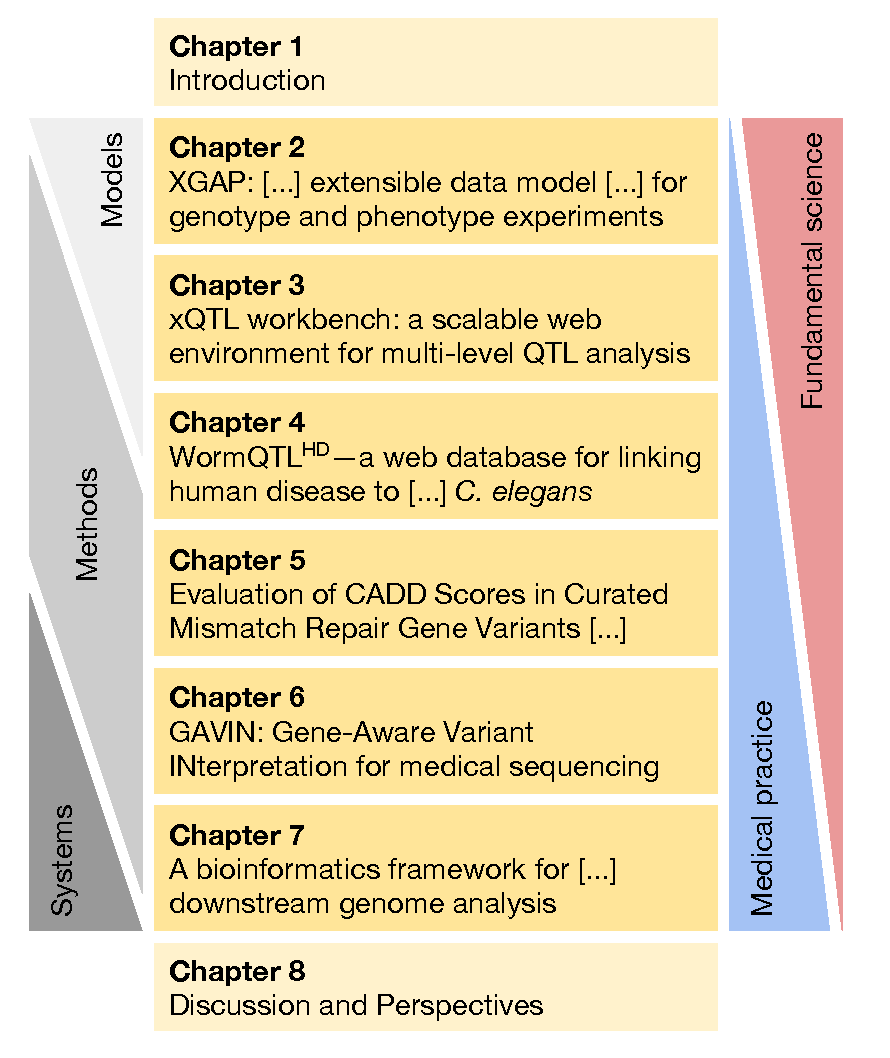
\includegraphics[width=1.0\linewidth]{img/introduction_chapters.eps}
\caption[Overview of thesis chapter progression]{Overview of thesis chapter progression in terms of type of output and area of application. We can define an overall gradient from fundamental science to medical practice, as well as transitions from models to integrate life science data towards methods to translate discovered knowledge and systems to implement new methods into patient care.}
\label{fig:introduction_chapters}
\end{figure}

\subsection[New models to integrate life science data]{New models to integrate life science data for genetic disease research (chapters \ref{chap:xgap} and \ref{chap:xqtl})}

There are many approaches for gathering, structuring, integrating and analyzing life science data, each best suited to test a spe\-ci\-fic hy\-po\-the\-sis\cite{Ritchie_2015}.
To help domain experts test new ideas and quickly interpret interesting findings, they should be able run the necessary queries, tools and visualizations themselves.
To achieve this, the underlying data has to be both properly modeled ('computer-readable') and fortified with enough metadata to describe what the data means\cite{Wilkinson_2016} so that it can be automatically addressed by applicable tools.

As data volumes grow ever larger, these tools have to be executed on external high-throughput computational environments such as multi-node computer clusters.
To facilitate storage of these huge datasets and parallelized computation, we investigated how to store complex data using the flexible XGAP model in chapter \ref{chap:xgap}, and used this as a basis to develop xQTL workbench in chapter \ref{chap:xqtl}.
xQTL workbench is a flexible database system designed to store any genotype and phenotype information with basic visualization and computational capabilities.

\subsection[New methods to translate research findings]{New methods to translate research findings to medical genetics (chapters \ref{chap:wormqtl} and \ref{chap:caddmmr})}

Translational medicine investigates how relevant new findings can be used to improve patient diagnosis and care.
To demonstrate how new findings can be generated, we loaded almost 100 data sets of \textsl{C. elegans} into an xQTL database, containing around 300 million measurements.
To show value for human health applications, we connected worm phenotypes to human disease at a molecular level using protein orthology.
Chapter \ref{chap:wormqtl} shows how these data can now be used to find models and leads for human disease research.
Furthermore, a biologist-friendly online environment enables the research community to join in and dig through the data.

Interesting findings need to be explored further and placed into clinical context before medical genetics can benefit from them.
The previously mentioned CADD scores\cite{Kircher_2014} are an example of an innovation with great potential.
Doctors and clinical geneticists have an interest in such developments, but cannot use it in practice without guidelines about how to interpret these scores in patient cases.
To explore how such a guideline is created and used, we translated CADD scores to the clinical classification of variants in mismatch repair genes in chapter \ref{chap:caddmmr}.
These genes may harbor variants that cause hereditary colorectal cancer.
By characterizing these scores in this context, we learned both their pitfalls and how they can be used to prioritize new mutations or double-check existing classifications.

\subsection[New systems for medical genetics practice]{New systems to implement methods into medical genetics practice (chapters \ref{chap:gavin} and \ref{chap:frameworkforgenomics})}

Large reference datasets and computational resources, when guided by translational research, should allow us to transform patient care.
To facilitate this, we need to design, build and maintain reliable software systems\cite{Prins_2015} running on a stable server and database infrastructure\cite{Swertz_2007}.
These systems must handle rapidly increasing quantities of whole-ge\-no\-me data as sequencing costs dropped from a billion dollars to just a thousand dollars per patient.
The data produced needs to be contrasted against large population reference sets and other patient genomes for research, interpretation or diagnosis using computational methods.
The storage, processing and filtering solutions for these massive datasets need the capabilities to be scaled up, fine-tuned and clinically validated accordingly.

Encouraged by results of chapter \ref{chap:caddmmr}, we generalized the CADD score calibration approach and applied it to $>$3,000 disease genes.
We emphasize practical use by excluding variants that would also excluded by existing methods.
On the variants that remain that are hard to interpret, we find out if CADD scores can be of further help.
The resulting predictor tool, GAVIN, is described in chapter \ref{chap:gavin} and works remarkably well for clinically characterized genes.
It serves as a first-lead causal variant screening tool with broad application in clinical genomics.

This work then feeds into chapter \ref{chap:frameworkforgenomics}, where we define a framework to automate the interpretation of genomic data, and to fast-track innovations in this process. 
We implement the GAVIN+ interpretation tool, which combines GAVIN with additional knowledge and criteria from clinical genetics to quickly identify variants and genotypes that are potentially disease-causing.
This tool outputs its result in the new rVCF (Report VCF) format, which captures any relevant analysis results along with detailed provenance information and the reason why a variant is of interest.

Using this format, we can run fast validation on known pathogenic variants and estimation of false discovery rate on healthy control samples.
The final result can be visualized in a customizable doctor-friendly report, analyzed further as the format is fully compliant with existing tools, and shared with peers.
The modular framework design separates the enrichment, interpretation and visualization of the data.

Our proposed solution is flexible and maintainable and its standardized formats allows the community to develop focused software tools that produce and utilize these files.
As a result, newly developed methods can be quickly adapted and validated within local installation of the framework.
This high-throughput infrastructure will speed up molecular diagnostic practice, and prepare it for seamless future integration of new analysis methods and powerful new omics techniques.
